\documentclass[12pt, titlepage]{article}

\usepackage{booktabs}
\usepackage{tabularx}
\usepackage{hyperref}

\usepackage{fullpage}
\usepackage[round]{natbib}
\usepackage{multirow}
\usepackage{booktabs}
\usepackage{tabularx}
\usepackage{graphicx}
\usepackage{float}
\usepackage{hyperref}
\usepackage{colortbl}
\usepackage[table]{xcolor} 
\hypersetup{
    colorlinks,
    citecolor=black,
    filecolor=black,
    linkcolor=red,
    urlcolor=blue
}
\usepackage[round]{natbib}

%% Comments

\usepackage{color}

%\newif\ifcomments\commentstrue %displays comments
\newif\ifcomments\commentsfalse %so that comments do not display

\ifcomments
\newcommand{\authornote}[3]{\textcolor{#1}{[#3 ---#2]}}
\newcommand{\todo}[1]{\textcolor{red}{[TODO: #1]}}
\else
\newcommand{\authornote}[3]{}
\newcommand{\todo}[1]{}
\fi

\newcommand{\wss}[1]{\authornote{blue}{SS}{#1}} 
\newcommand{\plt}[1]{\authornote{magenta}{TPLT}{#1}} %For explanation of the template
\newcommand{\an}[1]{\authornote{cyan}{Author}{#1}}

%% Common Parts

\newcommand{\progname}{Mechatronics Engineering} % PUT YOUR PROGRAM NAME HERE
\newcommand{\authname}{Team 25, Preliminary
\\ Ahmed Nazir, nazira1
\\ Stephen Oh, ohs9
\\ Muhanad Sada, sadam
\\ Tioluwalayomi Babayeju, babayejt} % AUTHOR NAMES                  

\usepackage{hyperref}
    \hypersetup{colorlinks=true, linkcolor=blue, citecolor=blue, filecolor=blue,
                urlcolor=blue, unicode=false}
    \urlstyle{same}
                                


\begin{document}

\title{Verification and Validation Report: \progname} 
\author{\authname}
\date{\today}
	
\maketitle

\pagenumbering{roman}

\section{Revision History}

\begin{tabularx}{\textwidth}{p{3cm}p{2cm}X}
\toprule {\bf Date} & {\bf Version} & {\bf Notes}\\
\midrule
Date 1 & 1.0 & Notes\\
Date 2 & 1.1 & Notes\\
\bottomrule
\end{tabularx}

~\newpage

\section{Symbols, Abbreviations and Acronyms}

\renewcommand{\arraystretch}{1.2}
\begin{tabular}{l l} 
  \toprule		
  \textbf{symbol} & \textbf{description}\\
  \midrule 
  T & Test\\
  \bottomrule
\end{tabular}\\

\wss{symbols, abbreviations or acronyms -- you can reference the SRS tables if needed}

\newpage

\tableofcontents

\listoftables %if appropriate

\listoffigures %if appropriate

\newpage

\pagenumbering{arabic}



\section{Functional Requirements Evaluation}
\subsection{Sensor Validation}
%sensor validation: Stephen
\begin{table}[H]
  \begin{tabular}{| p{0.15\textwidth} | p{0.10\textwidth}| p{0.28\textwidth}| p{0.28\textwidth}| p{0.09\textwidth}|}
    \hline
    \rowcolor[gray]{0.9}
    Test Number & Type & Input & Output & Result\\
    \hline
    ST-SV 1 & Manual & Room at a constant 25 $^{\circ}$C ambient & Constant 25.4 $^{\circ}$C reading from temperature sensor & Pass \\
    \hline
    ST-SV 2 & Manual & Room at constant 40\% humidity $^{\circ}$C & Constant 43\% reading from humidity sensor & Pass \\
    \hline
    ST-SV 3 & Manual & 4 seperate phonecalls with accelerometer measuring haptic feedback & Maximum error between acceleration profiles of phone calls within 0.2 meters per second squared & Pass  \\
    \hline
  \end{tabular}
  \caption{Sensor Validation}
  \end{table}

%device telemetry: Ahmed
\subsection{Device Telemetry}
\begin{table}[H]
  \begin{tabular}{| p{0.15\textwidth} | p{0.10\textwidth}| p{0.28\textwidth}| p{0.28\textwidth}| p{0.09\textwidth}|}
    \hline
    \rowcolor[gray]{0.9}
    Test Number & Type & Input & Output & Result\\
    \hline
    ST-DT 1 & Manual & The device is connected via Wi-Fi and the start button is pressed on the GUI & The device beings to send and display the sensor data in the GUI & Pass \\
    \hline
    ST-DT 2 & Manual & The device is connected via Wi-Fi and the start button is pressed multiple times in the GUI & The start button greys out not allowing the user to press it multiple times and the sensors still send data to the GUI & Pass \\
    \hline
    ST-DT 3 & Manual & The device is connected via Wi-Fi and the stop button is pressed on the GUI & The device stops sending data to the GUI & Pass  \\
    \hline
    ST-DT 4 & Manual & The device is connected via Wi-Fi and the stop button is pressed multiple times in the GUI & The stop button greys out not allowing the user to press it multiple times and the device does not send data & Pass  \\
    \hline
  \end{tabular}
  \caption{Device Telemetry}
  \end{table}

%device hardware: Stephen
\subsection{Device Hardware}
\begin{table}[H]
  \begin{tabular}{| p{0.15\textwidth} | p{0.10\textwidth}| p{0.28\textwidth}| p{0.28\textwidth}| p{0.09\textwidth}|}
    \hline
    \rowcolor[gray]{0.9}
    Test Number & Type & Input & Output & Result\\
    \hline
    ST-DH 1 & Manual & Temperature sensor male end JST connector unconnected to the device's female JST connector & Device measured the room's ambient temperature at 23.4 $^{\circ}$C & Pass \\
    \hline
    ST-DH 2 & Manual & Device collecting sensor data at low battery charge & Device unoperational upon battery depletion and halted sensor data collection & Fail \\
    \hline
    ST-DH 3 & Manual & 5 kg dumbbell placed on each corner of the device chassis & No plastic failure in device chassis & Pass  \\
    \hline
    ST-DH 4 & Manual & A member on the formula electric team was given a cross screwdriver, M4 screw, the device, and DIN rail & The formula electric team member mounted the device in 40 seconds & Pass  \\
    \hline
%REMEMBER TO DELETE ST-DH5 FROM VNVPLAN, WE DO NOT NEED THIS TEST AS WE DO NOT HAVE A SCREEN OR DEVICE STATUS MEASUREMENTS
  \end{tabular}
  \caption{Device Hardware}
  \end{table} 
 

  ST-DH3 failed the functional test case. The team estimated the time required to design and integrate a rechargeable battery subsystem within the project's timeline was 1.5 weeks and decided the effort was not worthwhile relative to other project objectives. As a result, the failure of this test case lead the expected operation at low battery to be adjusted. Users are now expected to replace the battery on a regular schedule to prevent a failure in test integrity due to charge depletion. \\

\newpage
%desktop app: Mo
\subsection{Desktop Application}
ST-DA3 and ST-DA4 are included in unit testing, refer to section 5.3 for further details.
\begin{table}[H]
\begin{tabular}{| p{0.15\textwidth} | p{0.10\textwidth}| p{0.28\textwidth}| p{0.28\textwidth}| p{0.09\textwidth}|}
  \hline
  \rowcolor[gray]{0.9}
  Test Number & Input & Expected Output & Actual Output & Result\\
  \hline
  ST-DA5 & User clicks on 'Start Test' button in 'View Test' page & Live data start to populate a table in the UI & Live measurement data is displayed in a table in the UI & pass \\
  \hline
\end{tabular}
\caption{Desktop Application}
\end{table}

%data analytics: Tio
\subsection{Data Analytics Website}
\begin{table}[H]
  \begin{tabular}{| p{0.15\textwidth} | p{0.10\textwidth}| p{0.28\textwidth}| p{0.28\textwidth}| p{0.09\textwidth}|}
    \hline
    \rowcolor[gray]{0.9}
    Test Number & Type & Input & Output & Result\\
    \hline
    ST-DAW 1 & Manual & The user was given a username and password to login into Power BI & The user was able to view all the different data that was being recorded during the test and previous tests as well & Pass\\
    \hline
    ST-DAW 2 & Manual & The user was given a fake username and password that is not authorized to view the data & The user was not able to view the Power BI dataset that was created to view all the different test data & Pass\\
    \hline
  \end{tabular}
  \caption{Data Analytics}
  \end{table} 

We created our Data Analytics Website through a visualization tool called Power Bi and tested it to see if we were able to connect to the database which contained all our data values. We able to get all the values of our data from the database since Power Bi has a method that can connect to database that authorized users are allowed to connect to. Since this was the case we were able to pass this this requirement for our the data analytics.


%database: Mo
\subsection{Database}
\begin{table}[H]
\begin{tabular}{| p{0.15\textwidth} | p{0.10\textwidth}| p{0.28\textwidth}| p{0.28\textwidth}| p{0.09\textwidth}|}
  \hline
  \rowcolor[gray]{0.9}
  Test Number & Input & Expected Output & Actual Output & Result\\
  \hline
  ST-D1 & User clicks on 'Submit' button in 'Submit Test' page consecutively in a short period of time & UI displays error message 'Too many submissions' in red & 'Too many submissions' is displayed in red & pass \\
  \hline
\end{tabular}
\caption{Database}
\end{table}

\section{Nonfunctional Requirements Evaluation}
\subsection{Usability}
%Stephen
%Need a graph (that we generate) that supports data
\begin{table}[H]
  \begin{tabular}{| p{0.15\textwidth} | p{0.10\textwidth}| p{0.28\textwidth}| p{0.28\textwidth}| p{0.09\textwidth}|}
    \hline
    \rowcolor[gray]{0.9}
    Test Number & Type & Input & Output & Result\\
    \hline
    ST-U 1-A & Manual & User connects a thermistor to device, begins collecting sensor test data and gathers data for 1 minute, completes collecting sensor test data, adds remarks to the test, and submits test data to database & User completed the overall process in 3 minutes 43 seconds and rated the sensor mount and measuring procedure a 5. All other categories were given a 4 & Pass \\
    \hline
    ST-U 1-B & Manual & User adjusts Arduino code for a fluid flow rate sensor, connects the sensor to the device, begins collecting sensor test data and gathers data for 1 minute, completes collecting sensor test data, adds remarks to the test, and submits test data to database & User completed the process in 49 minutes 15 seconds and rated the overall experience a 2. The sensor mount and measuring procedure categories were given a 5. All other cattegories were given a 4 & Fail \\
    \hline
    ST-U 2-A & Manual & Device collecting sensor data with wired connection to a laptop running the python application & Python application GUI displayed at minimal latency. Less than 1 second latency for changes in sensor measurements to display on GUI & Pass \\
    \hline
    ST-U 2-B & Manual & Device collecting sensor data with wireless connection to a laptop running the python application & Python application GUI displayed at minimal latency. Less than 1 second latency for changes in sensor measurements to display on GUI & Pass \\
    \hline

    ST-U 3-A & Manual & Device connection to application is broken. User submits previous test data held on the micro-SD module to the database & Test data submits and test contents can be viewed on dashboard & Pass \\
    \hline
    ST-U 3-B & Manual & Application connection to database is broken. User can connect a temperature sensor, start a test, and stop a test & Device recognizes sensor, starts test, and stops test & Pass  \\
    \hline
  \end{tabular}
  \caption{Usability}
  \end{table}

  \begin{figure}[htbp!]
    \begin{center}
    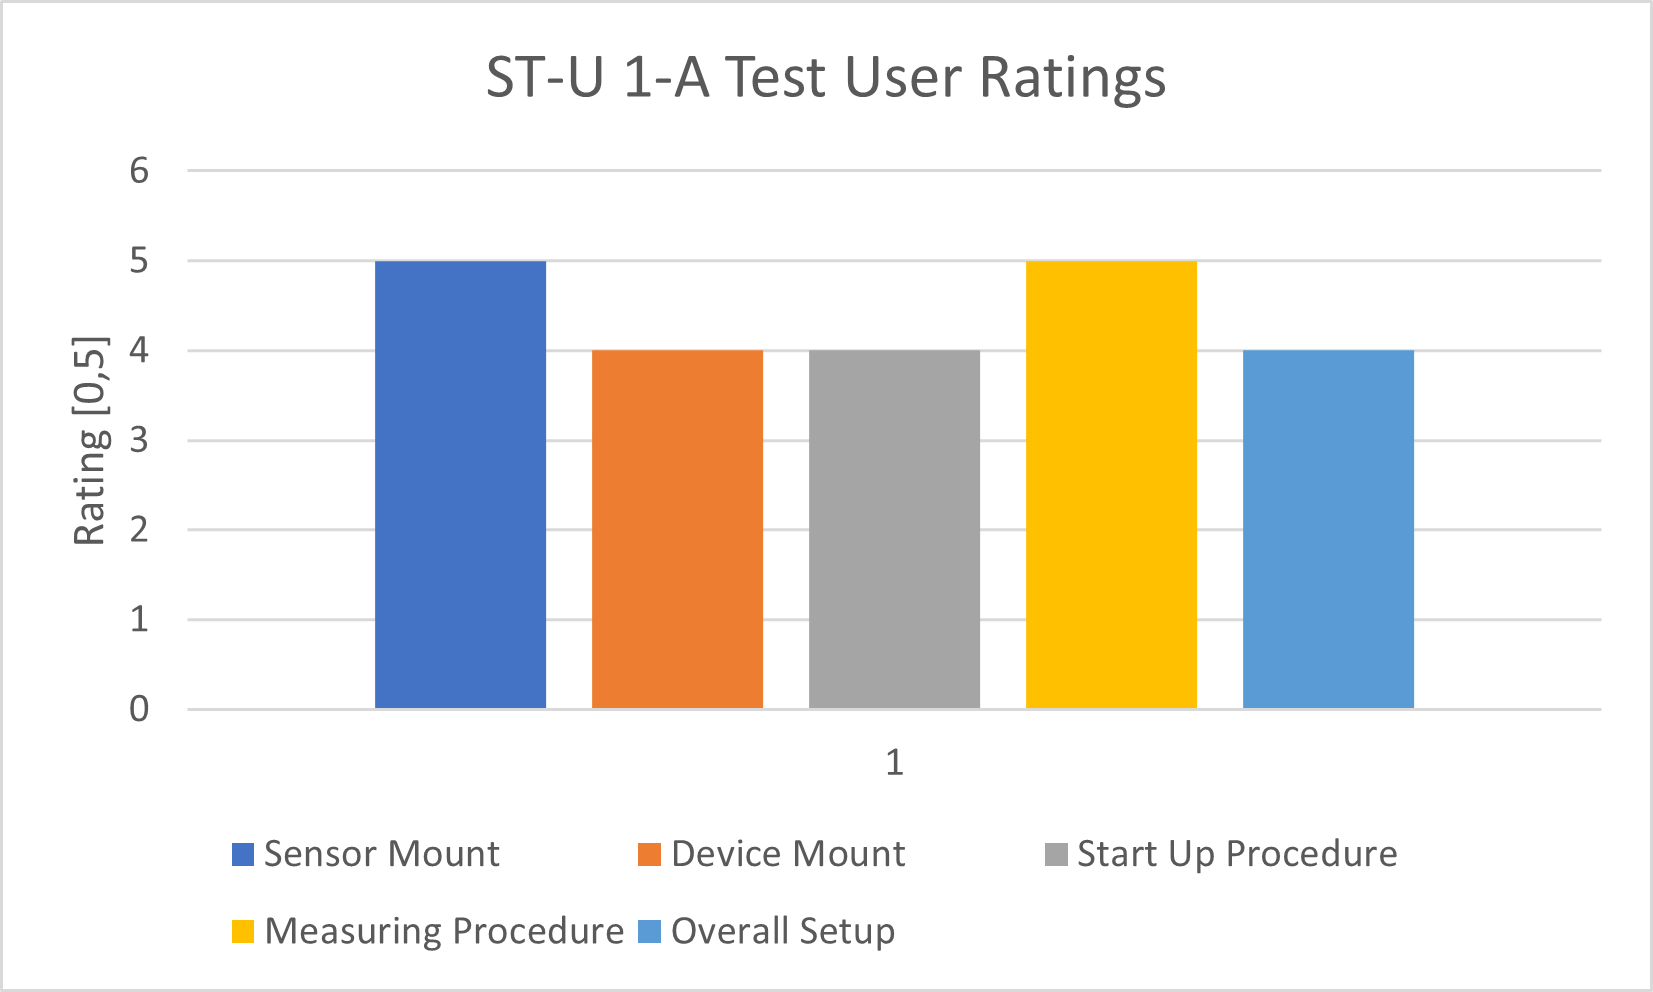
\includegraphics[width=0.8\textwidth]{ST-U_1-A_TestUserRatings}
    \caption{ST-U 1-A Test User Ratings}
    \end{center}
    \end{figure}

  \begin{figure}[htbp!]
    \begin{center}
    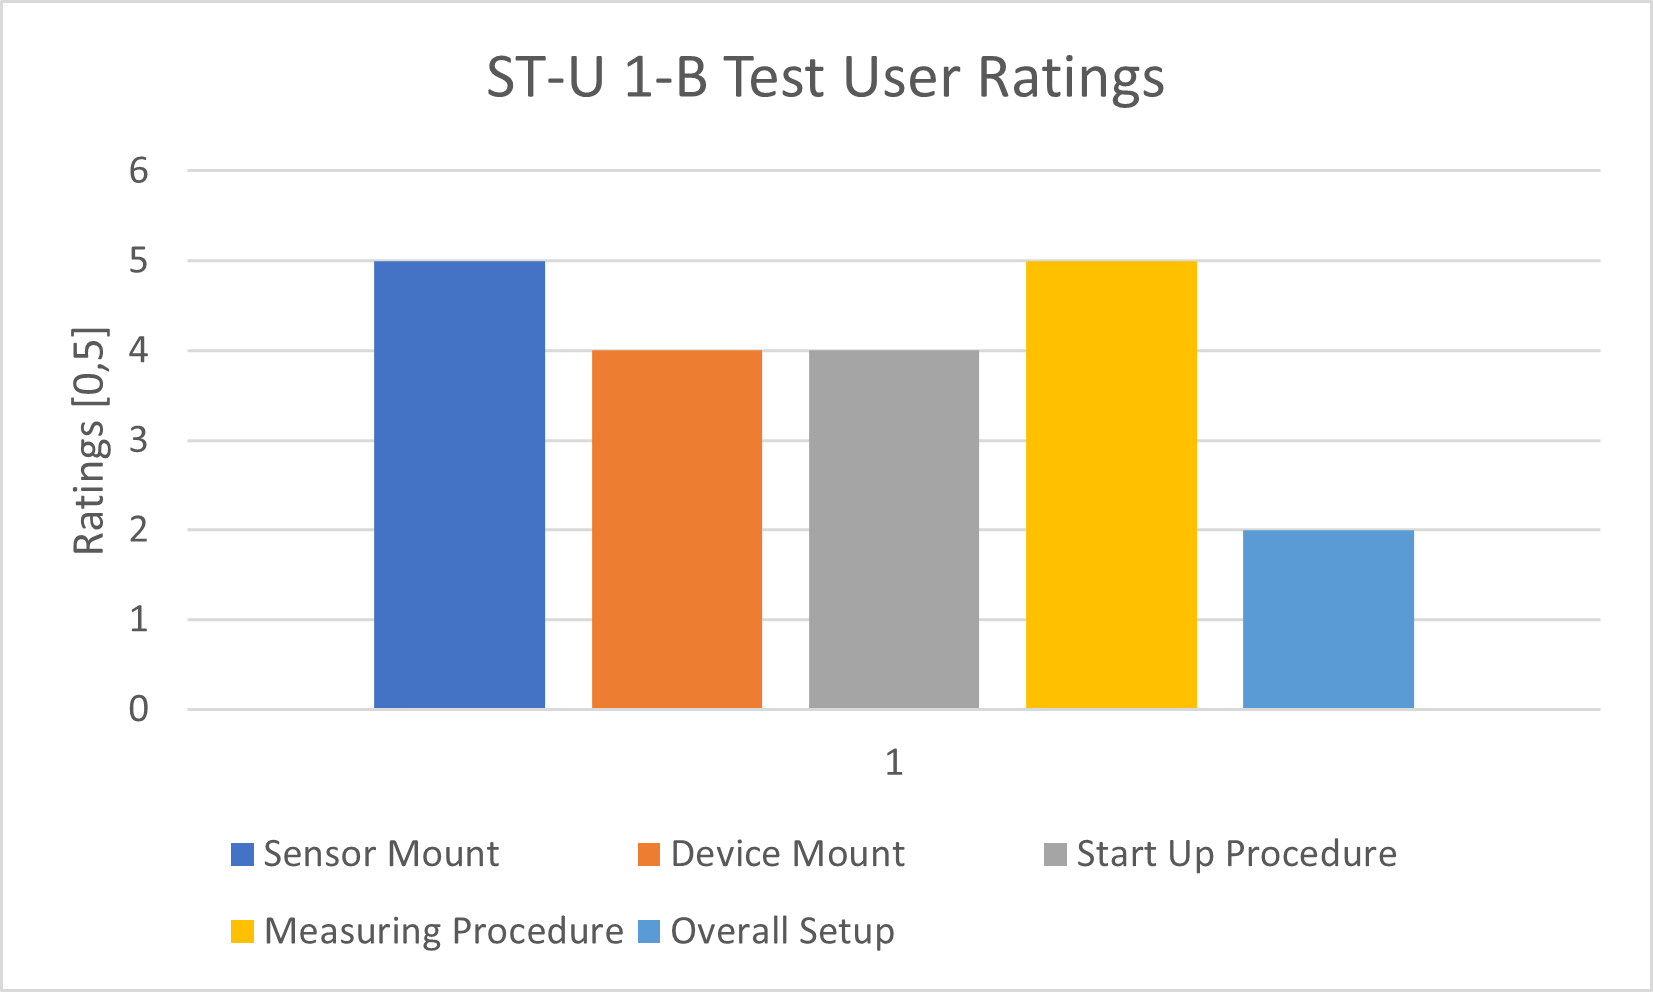
\includegraphics[width=0.8\textwidth]{ST-U_1-B_TestUserRatings}
    \caption{ST-U 1-B Test User Ratings}
    \end{center}
    \end{figure}

  ST-U 1-B failed the usability test case. The difference between ST-U 1-B and ST-U 1-A was the user requirement to adjust and write the Arduino code for a sensor not previously used with the device. Notably, the user experienced difficulty and was intimidated with adjusting existing code to integrate a new sensor. This effect was shown in both the increased time to complete the overall process and the decreased rating in the overall test experience category. As a result, the project will have an approach whereby the user should only interact with the graphical user interface to reduce the user's feelings of complexity and intimidation when integrating a new sensor. The goal is to abstract the adjustments in the backend when implementing a new sensor by having the user interact only with the GUI and following guided steps in plain English to fill in the required information to integrate a new sensor. \\


\subsection{Performance}
%Tio
\begin{table}[H]
  \begin{tabular}{| p{0.15\textwidth} | p{0.10\textwidth}| p{0.28\textwidth}| p{0.28\textwidth}| p{0.09\textwidth}|}
    \hline
    \rowcolor[gray]{0.9}
    Test Number & Type & Input & Output & Result\\
    \hline
    ST-P 1 & Dynamic, Manual & The device will be mounted and be tested in various conditions & The device was operational and stayed physcially intact after being tested in various conditions & Pass\\
    \hline
    ST-P 2 & Dynamic, Manual & The device will be operating and collecting data from a test and streaming the results to our desktop application & The latency between the collecting of data and the streaming of it remained below 10 seconds & Pass\\
    \hline
    ST-P 3 & Dynamic, Manual & The device will be operating with one or more of the connections to either the device, application and or database & The user is still able to obtain the test results of the current test no matter which connections are missing on the overall connection & Pass\\
    \hline
  \end{tabular}
  \caption{Performance}
  \end{table}

\subsection{Security}
%Tio
\begin{table}[H]
  \begin{tabular}{| p{0.15\textwidth} | p{0.10\textwidth}| p{0.28\textwidth}| p{0.28\textwidth}| p{0.09\textwidth}|}
    \hline
    \rowcolor[gray]{0.9}
    Test Number & Type & Input & Output & Result\\
    \hline
    ST-S 1 & Dynamic, Manual & User will receive numerous usernames and passwords and attempt to access the database & The database was only accessible using the correct username, password and only with specific ip addresses that have been accepted & Pass\\
    \hline
    ST-S 2 & Dynamic, Manual & Multiple fake data points were attempted to be added to the database & The database remained the same even after the attempted modification ensuring that only authorized were allowed to modify the database & Pass\\
    \hline
  \end{tabular}
  \caption{Security}
  \end{table}

\newpage
\section{Unit Testing}
\subsection{Module - ui\_functions.py}
%Desktop App Code: Mo
%Arduino Code: Ahmed
connect\_wireless(self) - Tested by clicking connect button on wireless page
\begin{table}[H]
  \begin{tabular}{| p{0.1\textwidth} | p{0.15\textwidth}| p{0.28\textwidth}| p{0.28\textwidth}| p{0.09\textwidth}|}
    \hline
    \rowcolor[gray]{0.9}
    Test No. & Input & Expected Output & Actual Output & Result\\
    \hline
    U1 & Connected to Formulate Wi-Fi & The application should connect to the device and display that it is connected & The application shows that the device is connected & Pass \\
    \hline
    U2 & Not Connected to Formulate Wi-Fi  & The application should display a pop up error indicating to the user that they need to connect to the Formulate Wi-Fi & A popup is displayed to the user to indicate they need to connect to Wi-Fi & Pass \\
    \hline
    U3 & -Connected to Formulate Wi-Fi -Device is connected via Serial (Wired) & The application should disconnect from serial and follow U1 & The application disconnects from serial and follows U1 & Pass \\
    \hline
  \end{tabular}
  \caption{Unit Test - connect\_wireless(self)}
  \end{table}

disconnect\_wireless(self) - Tested by clicking disconnect button on wireless page
\begin{table}[H]
  \begin{tabular}{| p{0.1\textwidth} | p{0.15\textwidth}| p{0.28\textwidth}| p{0.28\textwidth}| p{0.09\textwidth}|}
    \hline
    \rowcolor[gray]{0.9}
    Test No. & Input & Expected Output & Actual Output & Result\\
    \hline
    U4 & -Connected to Formulate Wi-Fi -The disconnect button is clicked & The application should disconnect from the board and display that it is disconnected & The application disconnects from board and shows its disconnected & Pass \\
    \hline
    U5 & Not Connected to Formulate Wi-Fi  & The application should not display the disconnect button on the connectivity widget & The application does not display the disconnect button & Pass \\
    \hline
  \end{tabular}
  \caption{Unit Test - disconnect\_wireless(self)}
  \end{table}

  connect\_wired(self) - Tested by clicking connect button on wired page
  \begin{table}[H]
    \begin{tabular}{| p{0.1\textwidth} | p{0.15\textwidth}| p{0.28\textwidth}| p{0.28\textwidth}| p{0.09\textwidth}|}
      \hline
      \rowcolor[gray]{0.9}
      Test No. & Input & Expected Output & Actual Output & Result\\
      \hline
      U6 & Connected to PC via USB and the correct COM port is selected in the Wire connectivity widget & The application should connect to the device and display that it is connected & The application shows that the device is connected & Pass \\
      \hline
      U7 & Not Connected to PC via wire  & The application should not display any COM port in the widget & The wired drop down is empty and shows no COM port & Pass \\
      \hline
      U8 & -Connected to PC via USB and the correct COM port is selected in the Wire connectivity widget -Device is connected via WiFi & The application should disconnect from WiFi and follow U6 & The application disconnects from WiFi and follows U6 & Pass \\
      \hline
    \end{tabular}
    \caption{Unit Test - connect\_wired(self)}
    \end{table}
  
  disconnect\_wired(self) - Tested by clicking disconnect button on wired page
  \begin{table}[H]
    \begin{tabular}{| p{0.1\textwidth} | p{0.15\textwidth}| p{0.28\textwidth}| p{0.28\textwidth}| p{0.09\textwidth}|}
      \hline
      \rowcolor[gray]{0.9}
      Test No. & Input & Expected Output & Actual Output & Result\\
      \hline
      U9 & -Connected via wired -The disconnect button is clicked & The application should disconnect from the board and display that it is disconnected & The application disconnects from board and shows its disconnected & Pass \\
      \hline
    \end{tabular}
    \caption{Unit Test - disconnect\_wired(self)}
    \end{table}
\newpage

  ping(self) - Tested by clicking connect button
  \begin{table}[H]
    \begin{tabular}{| p{0.1\textwidth} | p{0.15\textwidth}| p{0.28\textwidth}| p{0.28\textwidth}| p{0.09\textwidth}|}
      \hline
      \rowcolor[gray]{0.9}
      Test No. & Input & Expected Output & Actual Output & Result\\
      \hline
      U10 & Connected via WiFi & The application should read which sensors are flashed on the board and display them & The application gets which sensors are flashed and displays them & Pass \\
      \hline
      U11 & Connected via wired & The application should read which sensors are flashed on the board and display them & The application gets which sensors are flashed and displays them & Pass \\
      \hline
    \end{tabular}
    \caption{Unit Test - ping(self)}
    \end{table}

  startTest(self) - Tested by clicking startTest button
  \begin{table}[H]
    \begin{tabular}{| p{0.1\textwidth} | p{0.15\textwidth}| p{0.28\textwidth}| p{0.28\textwidth}| p{0.09\textwidth}|}
      \hline
      \rowcolor[gray]{0.9}
      Test No. & Input & Expected Output & Actual Output & Result\\
      \hline
      U12 & Connected via WiFi & The application should read data from the bytestring sent from the ESP8266 and display it in the table as the data is coming & The application reads the data and displays it correctly & Pass \\
      \hline
      U13 & Connected via wired & The application should read data from the bytestring sent from the Arduino UNO and display it in the table as the data is coming & The application reads the data and displays it correctly & Pass \\
      \hline
    \end{tabular}
    \caption{Unit Test - startTest(self)}
    \end{table}
\newpage
  stopTest(self) - Tested by clicking stopTest button
  \begin{table}[H]
    \begin{tabular}{| p{0.1\textwidth} | p{0.15\textwidth}| p{0.28\textwidth}| p{0.28\textwidth}| p{0.09\textwidth}|}
      \hline
      \rowcolor[gray]{0.9}
      Test No. & Input & Expected Output & Actual Output & Result\\
      \hline
      U14 & Connected via WiFi & The application should stop reading data sent from the ESP8266  & The application stops reading the data & Pass \\
      \hline
      U15 & Connected via wired & The application should stop reading data sent from the Arduino UNO & The application stops reading the data & Pass \\
      \hline
    \end{tabular}
    \caption{Unit Test - stopTest(self)}
    \end{table}

  declineData(self) - Tested by clicking stopTest button
  \begin{table}[H]
    \begin{tabular}{| p{0.1\textwidth} | p{0.15\textwidth}| p{0.28\textwidth}| p{0.28\textwidth}| p{0.09\textwidth}|}
      \hline
      \rowcolor[gray]{0.9}
      Test No. & Input & Expected Output & Actual Output & Result\\
      \hline
      U16 & There is data populated in the table & The application should clear all the data in the table and display an empty table  & The application clears the data and displays an empty table & Pass \\
      \hline
      U17 & There is no data populated in the table & The application should clear all the data in the table and display an empty table  & The application clears the data and displays an empty table & Pass \\
      \hline
    \end{tabular}
    \caption{Unit Test - declineData(self)}
    \end{table}

    setup\_page(self, page\_name) - Output observed in the UI \newline
\begin{table}[H]
  \begin{tabular}{| p{0.10\textwidth} | p{0.15\textwidth}| p{0.28\textwidth}| p{0.28\textwidth}| p{0.09\textwidth}|}
    \hline
    \rowcolor[gray]{0.9}
    Test No. & Input & Expected Output & Actual Output & Result\\
    \hline
    U18 & 'sign up page' & Sign up page has items added to the ‘team role’ dropdown and password/confirm password fields have hidden entry & Sign up page has items in ‘team role’ dropdown and password fields have the input hidden & pass \\
    \hline
    U19 & 'login page' & Login page’s password field entry is hidden & Login page’s password field entry is hidden & pass \\
    \hline
  \end{tabular}
  \caption{Unit Test - setup\_page}
\end{table}


login\_into\_app(self) - Tested by clicking 'Sign In' button in Login page of the UI \newline
\begin{table}[H]
  \begin{tabular}{| p{0.10\textwidth} | p{0.15\textwidth}| p{0.28\textwidth}| p{0.28\textwidth}| p{0.09\textwidth}|}
    \hline
    \rowcolor[gray]{0.9}
    Test No. & Input & Expected Output & Actual Output & Result\\
    \hline
    U20 & Signing in with correct user information and ‘admin’ user  & UI transitions to homepage and username is displayed in the top right corner  & UI transitioned to homepage and ‘admin’ was displayed in the top right corner & pass \\
    \hline
    U21 & Signing in with no password & UI displays error message ‘Please enter a password’ in red color & ‘Please enter a password’ is displayed in red & pass \\
    \hline
    U22 & Signing in with no username & UI displays error message ‘Please enter a username’ in red color & ‘Please enter a password’ is displayed in red & pass \\
    \hline
    U23 & Signing in with non-existing username & UI displays error message ‘User does not exist, try again’ in red color & ‘User does not exist, try again’ is displayed in red & pass \\
    \hline
    U24 & Signing in with incorrect password & UI displays error message ‘Incorrect password, try again’ in red color & ‘Incorrect password, try again’, is displayed in red & pass \\
    \hline
  \end{tabular}
  \caption{Unit Test - login\_into\_app}
\end{table}


continue\_signup(self) - Tested by clicking 'Continue' button in Sign Up page of the UI \newline
\begin{table}[H]
  \begin{tabular}{| p{0.10\textwidth} | p{0.15\textwidth}| p{0.28\textwidth}| p{0.28\textwidth}| p{0.09\textwidth}|}
    \hline
    \rowcolor[gray]{0.9}
    Test No. & Input & Expected Output & Actual Output & Result\\
    \hline
    U25 & Valid account registration information & UI transitions to homepage and new rows are added to Users and Login tables in database & UI transitioned to homepage and new rows with user information and hashed passwords were added to Users and Login tables in database & pass \\
    \hline
    U26 & At least one field is missing input & UI displays error message ‘Please fill in missing fields’ in red color & ‘Please fill in missing fields’ is displayed in red & pass \\
    \hline
    U27 & Username is less than 4 characters & UI displays error message ‘Username requires at least 4 characters’ in red color & ‘Username requires at least 4 characters’ is displayed in red & pass \\
    \hline
    U28 & Password is less than 8 characters & UI displays error message ‘Password requires at least 8 characters’ in red color & ‘Password requires at least 8 characters’ is displayed in red & pass \\
    \hline
    U29 & Password does not have a number & UI displays error message ‘Password requires at least one number’ in red color & ‘Password requires at least one number’ is displayed in red & pass \\
    \hline
    U30 & Password does not contain a letter & UI displays error message ‘Password requires at least one alphabet’ in red color & ‘Password requires at least one alphabet’ is displayed in red & pass \\
    \hline
    U31 & Password does not contain a non-alphanumeric character & UI displays error message ‘Password requires at least one non-alphanumeric character’ in red color & Correct error message is displayed but is cut off & fail \\
    \hline
    U32 & Password and Confirm Password fields do not match & UI displays error message ‘Passwords do not match’ in red color & ‘Passwords do not match’ is displayed in red & pass \\
    \hline
  \end{tabular}
  \caption{Unit Test - continue\_signup}
\end{table}

move\_to\_submit\_test(self): Tested by clicking on ‘Submit’ button in View Test page of the UI \newline
\begin{table}[H]
  \begin{tabular}{| p{0.10\textwidth} | p{0.15\textwidth}| p{0.28\textwidth}| p{0.28\textwidth}| p{0.09\textwidth}|}
    \hline
    \rowcolor[gray]{0.9}
    Test No. & Input & Expected Output & Actual Output & Result\\
    \hline
    U33 & Clicking on button while logged in & UI transitions to Submit Test page & UI transitioned to Submit Test page & pass \\
    \hline
    U34 & Clicking on button while not signed in & UI displays error message ‘Please login to submit tests’ & ‘Please login to submit tests’ is displayed & pass \\
    \hline
  \end{tabular}
  \caption{Unit Test - move\_to\_submit\_test}
\end{table}


browse\_and\_display\_pictures(self) - Tested by clicking on Upload Image button in Submit Test page of the UI \newline
\begin{table}[H]
  \begin{tabular}{| p{0.10\textwidth} | p{0.15\textwidth}| p{0.28\textwidth}| p{0.28\textwidth}| p{0.09\textwidth}|}
    \hline
    \rowcolor[gray]{0.9}
    Test No. & Input & Expected Output & Actual Output & Result\\
    \hline
    U35 & Described above & File explorer window pops up, user can select an image, and selected image is displayed in UI & The same as expected output & pass \\
    \hline
  \end{tabular}
  \caption{Unit Test - browse\_and\_display\_pictures}
\end{table}

upload\_test\_info(self) - Tested by clicking on 'Submit' button in Submit Test page of the UI \newline
\begin{table}[H]
  \begin{tabular}{| p{0.10\textwidth} | p{0.15\textwidth}| p{0.28\textwidth}| p{0.28\textwidth}| p{0.09\textwidth}|}
    \hline
    \rowcolor[gray]{0.9}
    Test No. & Input & Expected Output & Actual Output & Result\\
    \hline
    U36 & Valid data and test information provided & UI transitions to homepage and new test information should be visible in PowerBi dashboard & New test information was visibile in PowerBi dashboard & Pass \\
    \hline
    U37 & No test data & UI displays error message 'No data to submit' in red & 'No data to submit' was displayed in red & Pass \\
    \hline
    U38 & Valid test data but missing test name and/or purpose & UI displays error message 'Fill in missing fields' in red & 'Fill in missing fields' was displayed in red & Pass \\
    \hline
  \end{tabular}
  \caption{Unit Test - upload\_test\_info}
\end{table}


\subsection{Module - mainArduino.ino}\begin{table}[H]
  \begin{tabular}{| p{0.10\textwidth} | p{0.15\textwidth}| p{0.28\textwidth}| p{0.28\textwidth}| p{0.09\textwidth}|}
    \hline
    \rowcolor[gray]{0.9}
    Test No. & Input & Expected Output & Actual Output & Result\\
    \hline
    U39 & Device is connected via Wired and temperature sensor is connected & A bytestring of data in the form of (A1XX) should display & A bytestring of the correct form is displayed on the Arduino serial monitor & Pass \\
    \hline
    U40 & Device is connected via WiFi and temperature sensor is connected & A bytestring of data in the form of (A1XX) should display & A bytestring of the correct form is displayed on the Arduino serial monitor & Pass \\
    \hline
  \end{tabular}
  \caption{Unit Test - Arduino Bytestring}
\end{table}

\subsection{Module - mainESP8266.ino}\begin{table}[H]
  \begin{tabular}{| p{0.10\textwidth} | p{0.15\textwidth}| p{0.28\textwidth}| p{0.28\textwidth}| p{0.09\textwidth}|}
    \hline
    \rowcolor[gray]{0.9}
    Test No. & Input & Expected Output & Actual Output & Result\\
    \hline
    U41 & Device is connected to the Formulate WiFi & A Green LED should turn on & Green LED is turned on & Pass \\
    \hline
    U42 & Device is connected to Formulate WiFi and data is being transferred & An orange LED should turn on & A Orange LED is turned on & Pass \\
    \hline
  \end{tabular}
  \caption{Unit Test - ESP8266 Wireless Test}
\end{table}

  


\section{Changes Due to Testing}
%Each person will have to write a section here. Each FR and NFR will have a paragraph here, so based on what was assigned earlier, we will need to write a section here.

\subsection{Functional Requirements}
%NOTE: Only keep requirements in here that were changed
%FR 1 :
%Point 1: Changes
%Point 2: Effect the change had on project
FR 11 was changed such that the battery under expected operational use is non-rechargeable. Batteries will continue to be used but will change from rechargeable to non-rechargeable batteries with a scheduled replacement timeline close to charge depletion. This change followed the test ST-DH 2 results. \\

\subsection{Nonfunctional Requirements}

\wss{This section should highlight how feedback from the users and from 
the supervisor (when one exists) shaped the final product.  In particular 
the feedback from the Rev 0 demo to the supervisor (or to potential users) 
should be highlighted.}

Additional considerations to the GUI must be made in response to NFR1,  NFR2, and the test result ST-U 1-B. In particular, the team plans to improve the GUI to improve the user experience by minimizing and ultimately eliminating interaction with Arduino code when integrating new sensors and making the user work with the GUI to integrate new sensors. \\
		
\subsection{Unit Testing}
There was only one failed unit test case which was U31. The test case failed because the correct error message was being displayed but, it was cut off meaning only a portion of the error message was visible. In order to fix this, the size of the UI text window for the error message was increased and the result was that the UI now correctly displays the full message.
\section{Trace to Requirements}
%VnV Plan has this table
\begin{tabular}{| p{0.45\textwidth} | p{0.45\textwidth}|}
  \hline
  \rowcolor[gray]{0.9}
  Requirement & Test \\
  \hline
  FR 1 & ST-SV 1, ST-SV 2, ST-SV 3 \\
  \hline
  FR 2 & ST-DT 1, ST-DT 2, ST-DT 3, ST-DT 4 \\
  \hline
  FR 3 & ST-DT 1, ST-DT 2 \\
  \hline
  FR 4 & ST-DT 3, ST-DT 4 \\
  \hline
  FR 5 & ST-SV 1, ST-SV 2, ST-SV 3 \\
  \hline
  FR 6 & ST-DA 1 \\
  \hline
  FR 7 & ST-DA 3 ST-DA 4 \\
  \hline
  FR 8 & ST-DAW 1 \\
  \hline
  FR 9 & ST-DH 3 \\
  \hline
  FR 10 & ST-DH 4 \\
  \hline
  FR 11 & ST-DH 2 \\
  \hline
  FR 12 & ST-DT 1, ST-DT 2 \\
  \hline
  FR 14 & ST-DH 1 \\
  \hline
  FR 15 & ST-DA 5\\
  \hline
  FR 16 & ST-DH 5 \\
  \hline
  FR 17 & ST-DA 1 \\
  \hline
  FR 18 & ST-DA 2 \\
  \hline
  FR 19 & ST-DAW 2 \\
  \hline
  FR 20 & ST-DAW 1 \\
  \hline
  FR 21 & ST-DAW 1 \\
  \hline
  FR 22 & ST-D 1 \\
  \hline
  FR 23 & ST-DH 5 \\
  \hline
  NFR 1 & ST-U 1 ST-U 2 ST-U 3 \\
  \hline
  NFR 2 & ST-U 1 ST-U 2 ST-U 3 \\
  \hline
  NFR 3 & ST-P 2 \\
  \hline
  NFR 4 & ST-P 1 ST-P 3 \\
  \hline
  NFR 5 & ST-U 4 \\
  \hline
  NFR 6 & ST-P 1 \\
  \hline
  NFR 7 & ST-P 3 \\
  \hline
  NFR 8 & ST-U 2 \\
  \hline
  NFR 9 & ST-S 1 ST-S 2 \\
  \hline
\end{tabular}
		



\newpage{}
\section*{Appendix --- Reflection}

\wss{The information in this section will be used to evaluate the team members on the
graduate attribute of Reflection.  Please answer the following question:

  In what ways was the Verification and Validation (VnV) Plan different
  from the activities that were actually conducted for VnV?  If there were
  differences, what changes required the modification in the plan?  Why did
  these changes occur?  Would you be able to anticipate these changes in future
  projects?  If there weren't any differences, how was your team able to clearly
  predict a feasible amount of effort and the right tasks needed to build the
  evidence that demonstrates the required quality?  (It is expected that most
  teams will have had to deviate from their original VnV Plan.)}

 %Tio
  In our Verification and Validation Plan we had planned to create a website containing all the information and test data received throughout various tests by Mac Formula Electric. The website will organize data and help the user analyze it as well. We ultimately decided to use Power Bi, which is an interactive data visualization software that all McMaster students can access. We used Power Bi to meet our data visualization requirements as it helped improved user ease of use and compatibility with the database where our test data was being stored. We were able to verify that using Power Bi worked for our data analytics portion because the members of the Mac Formula Electric were able to use the visualized test data to aid them in future designs.\\

 %Stephen  
 The Verification and Validation Plan for usability differed from the actual activities conducted in the VnV. For example, the usability test ST-U 1 did not originally account for sensor code integration by the user during the test. But during VnV, the team realized that we needed to know both the total process time taken when the user already had the required code and when the user had to integrate the code to adequately determine the project's ability to meet the FR's and NFR's defined in the SRS. In the future, prototyping earlier in the design process can help identify important test cases when generating the VnV Plan. \\  %End of paragraph

 %Ahmed  
 For the most part, our VnV plan the physical device and embedded code was closely aligned with the actual VnV activities we conducted. During the VnV planning session, our team worked diligently to clearly outline the specific objectives and requirements for our final product. We conducted extensive research, and actively engaged with Formula Electric team members to gain a deeper understanding of the type of device they were looking for. This helped us develop a comprehensive VnV plan that was tailored to the specific needs and expectations of the project. While there were some changes to the plan as we progressed, the core elements were largely unchanged. This was due to a thorough planning process and our ability to anticipate potential challenges or modifications that might arise over the course of the project. Ultimately, this allowed us to execute our VnV activities with precision and confidence, and to demonstrate the high level of quality that was required for the final product. \\

  %Mo 
  After unit, desktop application, and database testing, the GUI verification activities were different from the plan in a variety of ways. Firstly, there was no unit testing in the plan because it was too early in the project to determine modules and units therefore, most test cases for unit testing were new. Secondly, some desktop application and database system tests mentioned in the plan were not applicable because some features were changed or not added. During UI implementation, it was possible to anticipate those changes in future projects but it would depend on the nature of the project. In this case, the project's UI was modified greatly from initial design to implementation. However, since some backend features of the project changed, it is completely normal for the verification to be also modified to accommodate the new or edited features of the UI.


\end{document}